\begin{figure}[h]
    \centering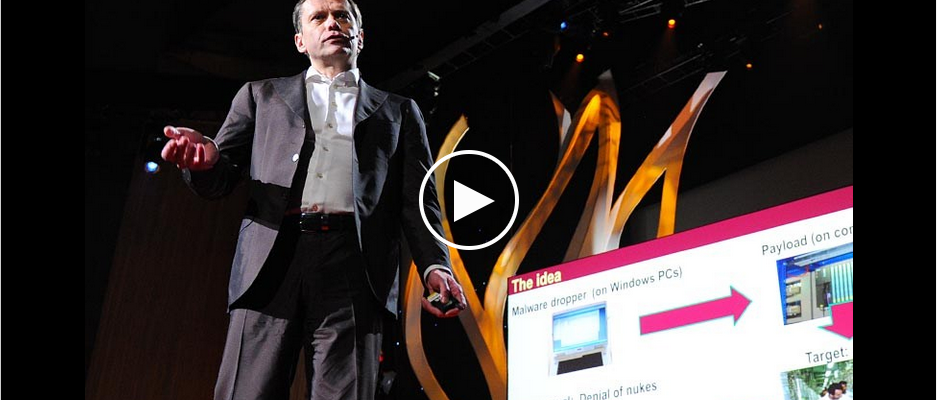
\includegraphics[scale=0.5]{stuxnet.png}
    \caption{\url{http://www.ted.com/talks/ralph\_langner\_cracking\_stuxnet\_a\_21st\_century\_cyberweapon}}
\end{figure}
Compromised systems that controlls centrifuges. Targeted Nucelar engineers.
that works on the systems. Payload is very complex. Looks for system calls, 
because their behaviour is know, Looks for timers and data structures. Smaller
payload seems designed to slowly crack centrifuge rotors. Big payload 
manipulates valves. Intercepts values from sensors, and gives fake input data. 
The idea is to circumvent digital safety systems. For more information on 
Stuxnet see:\\
\begin{enumerate}
    \item \url{https://en.wikipedia.org/wiki/Stuxnet}
    \item \url{https://archive.today/WS5uA}
    \item \url{http://go.eset.com/us/resources/white-papers/Stuxnet\_Under\_the\_Microscope.pdf}
    \item \url{http://www.symantec.com/content/en/us/enterprise/media/security\_response/whitepapers/w32\_stuxnet\_dossier.pdf}
\end{enumerate}

\textit{Digital evidence, evidence integrity and evidence dynamics}. 
We define digital evidence as any digital data that contains reliable 
information that supports or refutes a hypothesis about an incident.
Evidence integrity refers to the preservation of the evidence in its original 
form. This is a requirement that is valid both for the original evidence and the
image. Evidence dynamics is described to be any influence that changes, 
relocates, obscures, or obliterates evidence, regardless of intent.

\textit{Chain of custody and forensic soundness} - Chain of custody refers to 
the documentation of evidence acquisition, control, analysis and disposition 
of physical and electronic evidence. The term forensically sound methods and 
tools usually refers to the fact that the methods and tools adhere to best 
practice and legal requirements.

\textit{OOV} - Collect the most volatile data first – this increases the 
possibility to capture data about the incident in question. BUT: As you capture 
data in one part of the computer, you’re changing data in another

\textit{Evidence acquisition and verification} - For digital forensics it is typically
copy the data to a secure store, and then verify that the copy is
identical.

\textit{Cybercrime convention} - International agreement to increase cooperation
between countries. Criminal Law so things should be illeagal in all
countries. Criminal Procedure law, what police can do and how they do it.
Internet is borderless so there needs to be a effective cooperation
between countries to catch the bad guys.

\textit{Uncertanties in internet tracing} - Traffic is routed, so you do not
know if is original, anon traffic, time limits. TOR, VPN, proxies etc.

\subsection{File System Forensics}
\begin{figure}[h]
    \centering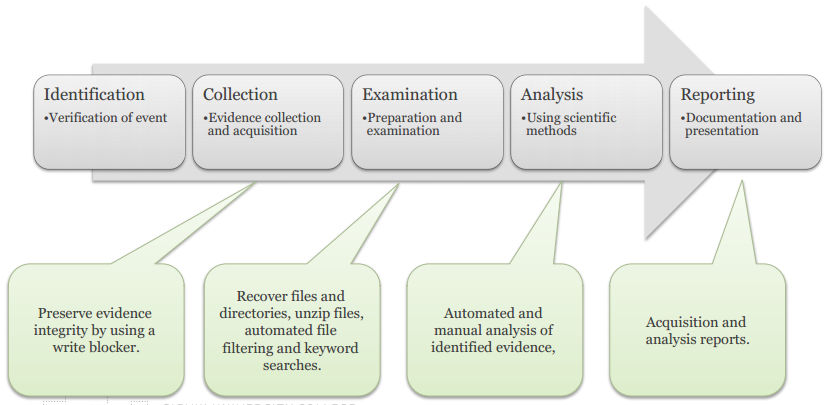
\includegraphics[scale=0.5]{fs_forensics.png}
\end{figure}
\begin{figure}[h]
    \centering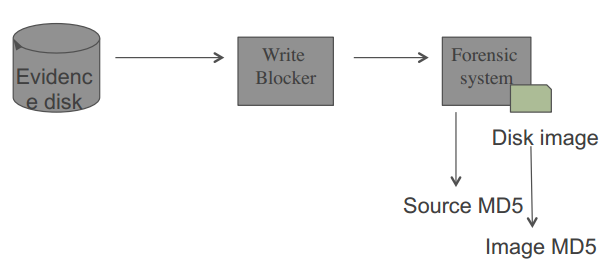
\includegraphics[scale=0.5]{disk_img.png}
\end{figure}

Forensic soundness and evidence integrity are critical, if a disk is found that
you belive contains evidence you need to make sure that any copy is forensically
sound, and the integrity of the evidence is preserved. To do this you connect
the disk to a write blocker. Write blockers are devices that allow acquisition 
of information on a drive without creating the possibility of accidentally 
damaging the drive contents. They do this by allowing read commands to pass but 
by blocking write commands, hence their name.
There are two ways to build a write-blocker: the blocker can allow all commands 
to pass from the computer to the drive except for those that are on a particular
list. Alternatively, the blocker can specifically block the write commands and 
let everything else through.
Write blockers may also include drive protection which will limit the speed of a
drive attached to the blocker. Drives that run at higher speed work harder(the 
head moves back and forth more often due to read errors). This added protection 
could allow drives that can not be read at high speed (UDMA modes) to be read at 
the slower modes (PIO).
There are two types of write blockers, Native and Tailgate. A Native device uses 
the same interface on for both in and out, for example a IDE to IDE write block. 
A Tailgate device uses one interface for one side and a different one for the 
other, for example a Firewire to SATA write block.
\footnote{http://www.forensicswiki.org/wiki/Write\_Blockers}
Hardware write blockers can be either IDE-to-IDE or Firewire/USB-to-IDE. 
Simson prefers the IDE-to-IDE because they deal better with errors on the drive 
and make it easier to access special information that is only accessible over 
the IDE interface.
Software write blockers can be either tailored to an individual operating system
or can be an independent boot disk. Their main upsides are with ease of use, 
since they are on a CD and do not require you to open up the case, and speed 
since they do not become a bottle neck.\\

There are many different types of media where digital evidence can be found, the
most obvious one is the disk, which there in turn are different types of. Today
we have the old HDD which are magnetic disks, and the newer SSDs and they pose
different challenges for the forensic analyst. On HDDs deleted data will persist
for a long time  if it is not overwritten, and the deleted data can easily be 
found when cloning the drive. Solid State Drives pose a variety of interesting 
challenges for computer forensics in comparison with traditional rotating 
magnetic platter hard drives. Most SSD devices are based on flash memory; some 
have battery backed SRAM or DRAM with a flash backing store. Flash has a number 
of key properties that complicate its use in computer storage systems and 
subsequent forensic analysis:\footnote{http://www.forensicswiki.org/wiki/Solid\_State\_Drives}
\begin{enumerate}
    \item Internally, flash memory is not divided into the traditional 512 byte 
        blocks, but instead is in pages of 2KiB, 4KiB, or larger, although it is
        still presented to the host computer in blocks

    \item Whilst hard drives can be written in a single pass, flash memory pages
        must be erased (in whole) before they can be rewritten

    \item Rewriting a block at the operating system level does not necessarily 
        rewrite the same page in the flash memory due to the controller 
        remapping data to spread wear or avoid failing pages

    \item Each page can be erased and rewritten a limited number of times – 
        typically 1000 to 10,000. (Hard drive sectors, in contrast, can be 
        rewritten millions of times or more.)

    \item Flash data is often encrypted on the drive, and can be "erased" by
        telling the controller to forget the old key and generate a new one, as
        well as marking all blocks as unused
\end{enumerate}

The controller in a flash SSD is significantly more complex in the number of 
tasks it has to perform in comparison to a magnetic rotating drive, with the 
following features:

\begin{enumerate}
    \item \textit{wear leveling} – that is, spreading the writes to flash out 
        among different sectors. Wear leveling is typically done with a flash 
        translation layer that maps logical sectors (or LBAs) to physical pages.
        Most FTLs are contained within the SSD device and are not accessible to 
        end users.

    \item \textit{read/modify/relocate+write} - if the controller allows 
        rewriting of a partial flash page, it must read the entire page, modify 
        the sector that is being written, and write the new flash page in a 
        new/fresh location which has been previously erased. the old 
        pre-modification data's page is then queued for erase.
\end{enumerate}
There are also a wide range of other media that can store digital evidence, such
as USB sticks, CDs, DVDs, Floppies, and a thousand other things. If the media is
encrypted and is powered down you are fucked if you do not know the key. If the
media is powered on and is in use there are ways to extract the key.
\footnote{https://en.wikipedia.org/wiki/Cold\_boot\_attack} A thing to note 
disk is the \textit{Host Protected Area} (HPA) which can be used to block a OS
from accessing the end of a drive. For more information about HPA see the 
footnote.\footnote{https://en.wikipedia.org/wiki/Host\_protected\_area}

\subsection{DOS Partitions}
DOS-based partitions are used by all x86 systems. The first 512 bytes of the
partition is the MBR. MBR contains boot code (0x0000), partition table (0x01BE)
, and a signature value (0x01FE).
\footnote{https://en.wikipedia.org/wiki/Master\_boot\_record}
The partition table contains four entries, each of which can describe a DOS 
partition. Addressing information, Number of sectors in partition, Type of 
partition, Flags. Example of partition types (0x01 - FAT12, 0x05 - Extended, 
0x07 - NTFS, 0x0C - FAT32, 0x0E FAT16, 0x83 - Linux Native, 0xA5 - BSD/386 ).

\subsection{Disk Analysis}
\begin{figure}[h]
    \centering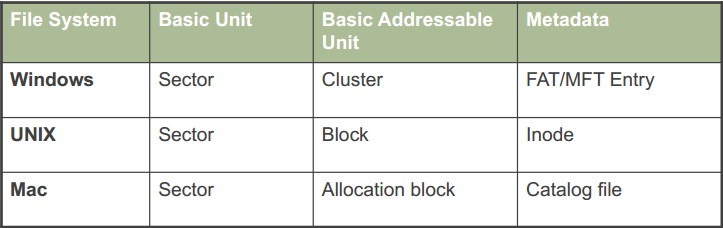
\includegraphics[scale=0.5]{disk_data_units.png}
\end{figure}
A block/cluster can be either allocated or unallocated. Allocated 
blocks/clusters are in use by a file and the data exists in a file on the file 
system. Unallocated blocks/clusters are not in use by any files, but they may 
contain deleted or unused data. Slackspace can be found at the end of sectors or
at the end of blocks/clusters. This occurs when a file does not fill its entire 
last sector or block/cluster. Note that most systems pad the end of the last 
sector of a file, but not the last blocks/clusters. There are two types of
slackspace, type 1 is unused part of a sector, and type 2 is a unused block
in a cluster. Slackspace and unallocated blocks are sources for deleted data.
\begin{figure}[h]
    \centering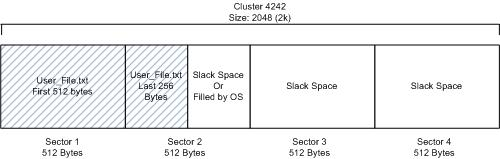
\includegraphics[scale=1]{slack_space.jpg}
\end{figure}

\subsection{Windows Metadata}
FAT directory entries: file name, long file name, MAC times (modification, 
access, creation), file size, first cluster number. NTFS: Master File Table
(MFT) entries: Standard information, file name, data. When deletining files on a
FAT system the file name minus the first letter is preserved, MAC times are 
preserved, file type, size etc are preserved. The clusters will be marked as 
unallocated but the data will be preserved. On NTFS nothing is tuched, but the
clusters are marked as unallocated. 

\subsection{UNIX Metadata}
UNIX file systems are organized within a single tree struture underneath one 
root directory. Disk partitions are mounted at some directory in the file 
system tree. A directory is organized as a sequence of directory entries. It 
contains File name and Inode number. Metadata is stored in the inode blocks,
some metadata is: ownership, permissions, file type, hard link count, file size
in bytes, time stamps (MAC, birth, deletion), Data block addresses (direct, 
single indirect, double indirect, \ldots). When a file is deleted, the directory
entry and inodenumber is marked as unused. The directory’s last MACtimes are set
to the time of the update. The inode block is marked as unused in the inode 
allocation bitmap. The file data blocks are marked as unused in the data block 
allocation bitmap, but the contents are left alone.



\subsection{Live Forensics}
Sometime you got to collect the evidence live on the computer, a typicall 
case is when you belive there is encryption involved. If the system is powered
down and you do not know they key then you are left with bruteforce attacks. 
Live forensics also give you access to other information that cannot else be
found such as running applications (something might be entered into the 
application that is not saved to disk). Active network connections, and if the
computer has been comprimised a lot of the information will be in the system
state. When doing live forensics you have to consider some things such as the
order of votality, you have to prioritize what data you want, because if you
access some of it it will affect some other data. You will also need to bring
the tools you need to use, as you cannot trust the information from the system.
If the computer is compromised and there is a rootkit present or some other 
piece of malware, then they can alter the information that is returned from
system tools. Memory can be found in many sources, such as RAM swap space and
hibernation files.

\begin{figure}[h]                                                                                                                 
    \centering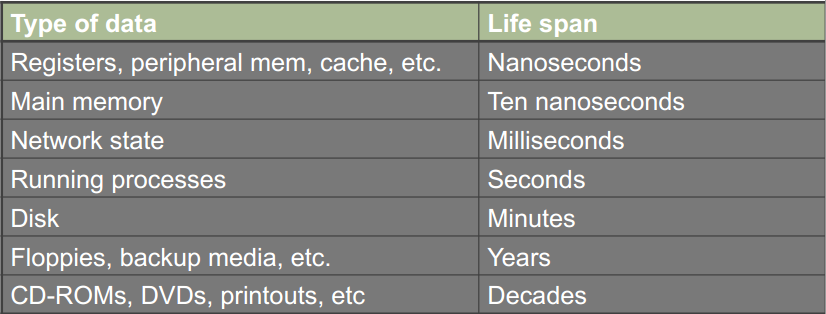
\includegraphics[scale=0.5]{oov.png}
    \caption{Table showing the life time of the different data types}
\end{figure}

\subsection{Remote Foresincs}
    Get data a from a remote computer.
    Think about secure channels, not good to copy thing in plaintext
    over the net.


